
\documentclass[11pt,oneside]{article} 

\usepackage{a4wide}

\usepackage{amsmath}
\usepackage{color}
%\usepackage{natbib} % kills arxiv 
\usepackage{framed}
%\usepackage{cite}
\usepackage{tikz}
\usepackage{tikz-cd}

% http://www.maths.qmul.ac.uk/~mf/genyoungtabtikz.sty
\usepackage[vcentermath]{genyoungtabtikz}
\Yboxdim{8pt}
%\Ylinethick{1pt}

\RequirePackage{amsmath}
\RequirePackage{amssymb}
\RequirePackage{amsthm}

%\RequirePackage{algorithmic}
%\RequirePackage{algorithm}
%\RequirePackage{theorem}
%\RequirePackage{eucal}
\RequirePackage{color}
\RequirePackage{url}
\RequirePackage{mdwlist}

\RequirePackage{rotating}


\RequirePackage[all]{xy}
%\_CompileMatrices
%\RequirePackage{hyperref}
\RequirePackage{graphicx}
%\RequirePackage[dvips]{geometry}

\usepackage{xcolor}
%\usepackage{amsmath,amsfonts,amssymb}
\usepackage{graphicx}
\usepackage[caption=false]{subfig}
\usepackage{enumerate}
\usepackage{mathrsfs}
\usepackage{bbm}

% -------------- Commands ----------------------

\makeatletter
\newcommand{\verbatimfont}[1]{\renewcommand{\verbatim@font}{\ttfamily#1}}
\makeatother

\newcommand{\Eref}[1]{(\ref{#1})}
\newcommand{\Fref}[1]{Fig.~\ref{#1}}
%\newcommand{\Aref}[1]{Appendix~\ref{#1}}
\newcommand{\SRef}[1]{Section~\ref{#1}}

\newcommand{\todo}[1]{\ \textcolor{red}{\{#1\}}\ }

\newcommand{\Aut}{\mathrm{Aut}}
\newcommand{\Hom}{\mathrm{Hom}}
%\newcommand{\hom}{\mathrm{hom}} % internal hom ?
\newcommand{\Stab}{\mathrm{Stab}}
\newcommand{\Fix}{\mathrm{Fix}}
\newcommand{\Orbit}{\mathrm{Orbit}}
\newcommand{\Ker}{\mathrm{Ker}}
\newcommand{\Image}{\mathrm{Im}}
\newcommand{\Dim}{\mathrm{Dim}}
\newcommand{\Complex}{\mathbb{C}}
\newcommand{\Integer}{\mathbb{Z}}
\newcommand{\Natural}{\mathbb{N}}

\newcommand{\GL}{\mathrm{GL}}
\newcommand{\SL}{\mathrm{SL}}
\newcommand{\SO}{\mathrm{SO}}
\newcommand{\Sp}{\mathrm{Sp}}
\newcommand{\PGL}{\mathrm{PGL}}
\newcommand{\Field}{\mathbb{F}}

\newcommand{\hsp}{\ \ \ \ }

% Lemma, proof, theorem, etc.
\newcommand\nounderline[1]{ #1} 
\newcommand\dodef[1]{\vskip 5pt \noindent{\bf \underline{Definition #1.}\ }}
\newcommand\dolemma[1]{\vskip 5pt \noindent{\bf \underline{Lemma #1.}\ }}
\newcommand\doproposition[1]{\vskip 5pt \noindent {\bf \underline{Proposition #1.}\ }}
\newcommand\dotheorem[1]{\vskip 5pt \noindent {\bf \underline{Theorem #1.}\ }}
\newcommand\docorollary[1]{\vskip 5pt \noindent {\bf \underline{Corollary #1.}\ }}
\newcommand\doexample[1]{\vskip 5pt \noindent {\bf \underline{Example #1.}\ }}
\newcommand\doproof{\vskip 5pt \noindent{\bf \nounderline{Proof:}\ }}

\newcommand\tombstone{\rule{.36em}{2ex}\vskip 5pt}

\newcounter{numitem}
\newcommand{\numlabel}[1]{\refstepcounter{numitem}\thenumitem\label{#1}}
\newcommand{\numitem}{\refstepcounter{numitem}\thenumitem}

% Categories
\newcommand{\Set}{\mathbf{Set}}
\newcommand{\FinSet}{\mathbf{FinSet}}
\newcommand{\GSet}{\mathbf{GSet}}
\newcommand{\GRep}{\mathbf{GRep}}
\newcommand{\CRing}{\mathbf{CRing}}

\newcommand{\thinplus}{\!+\!}

\newcommand{\tensor}{\otimes}

%
\newcommand{\DynkinAn}{
  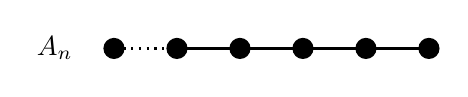
\begin{tikzpicture}[scale=.4]
    \draw (-1,0) node[anchor=east]  {$A_n$};
    \foreach \x in {0,...,5}
    \draw[xshift=\x cm,thick,fill=black] (\x cm,0) circle (.3cm);
    \draw[dotted,thick] (0.3 cm,0) -- +(1.4 cm,0);
    \foreach \y in {1.15,...,4.15}
    \draw[xshift=\y cm,thick] (\y cm,0) -- +(1.4 cm,0);
  \end{tikzpicture}
}

\newcommand{\DynkinAa}{
  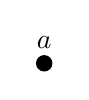
\begin{tikzpicture}[scale=.3]
    \draw (0,0.2) node[anchor=south] {$a$};
    \foreach \x in {0}
    \draw[xshift=\x cm,thick,fill=black] (\x cm,0) circle (.3cm);
  \end{tikzpicture}
}

\newcommand{\DynkinAab}{
  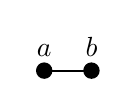
\begin{tikzpicture}[scale=.3]
    \draw (0,0.2) node[anchor=south] {$a$};
    \draw (2,0.2) node[anchor=south] {$b$};
    \foreach \x in {0,1}
    \draw[xshift=\x cm,thick,fill=black] (\x cm,0) circle (.3cm);
    \foreach \y in {0.15,...,0.15}
    \draw[xshift=\y cm,thick] (\y cm,0) -- +(1.4 cm,0);
  \end{tikzpicture}
}

\newcommand{\DynkinAabc}{
  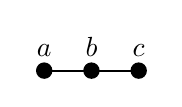
\begin{tikzpicture}[scale=.3]
    \draw (0,0.2) node[anchor=south] {$a$};
    \draw (2,0.2) node[anchor=south] {$b$};
    \draw (4,0.2) node[anchor=south] {$c$};
    \foreach \x in {0,1,2}
    \draw[xshift=\x cm,thick,fill=black] (\x cm,0) circle (.3cm);
    \foreach \y in {0.15,...,1.15}
    \draw[xshift=\y cm,thick] (\y cm,0) -- +(1.4 cm,0);
  \end{tikzpicture}
}

\newcommand{\DynkinAabcd}{
  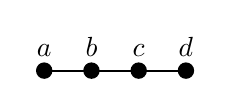
\begin{tikzpicture}[scale=.3]
    \draw (0,0.2) node[anchor=south] {$a$};
    \draw (2,0.2) node[anchor=south] {$b$};
    \draw (4,0.2) node[anchor=south] {$c$};
    \draw (6,0.2) node[anchor=south] {$d$};
    \foreach \x in {0,1,2,3}
    \draw[xshift=\x cm,thick,fill=black] (\x cm,0) circle (.3cm);
    \foreach \y in {0.15,...,2.15}
    \draw[xshift=\y cm,thick] (\y cm,0) -- +(1.4 cm,0);
  \end{tikzpicture}
}


\newcommand{\DynkinBn}{
  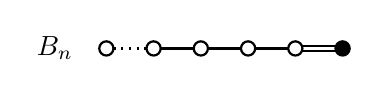
\begin{tikzpicture}[scale=.3]
    \draw (-1,0) node[anchor=east]  {$B_n$};
    \foreach \x in {0,...,4}
    \draw[xshift=\x cm,thick] (\x cm,0) circle (.3cm);
    \draw[xshift=5 cm,thick,fill=black] (5 cm, 0) circle (.3 cm);
    \draw[dotted,thick] (0.3 cm,0) -- +(1.4 cm,0);
    \foreach \y in {1.15,...,3.15}
    \draw[xshift=\y cm,thick] (\y cm,0) -- +(1.4 cm,0);
    \draw[thick] (8.3 cm, .1 cm) -- +(1.4 cm,0);
    \draw[thick] (8.3 cm, -.1 cm) -- +(1.4 cm,0);
  \end{tikzpicture}
}

\newcommand{\DynkinBab}{
  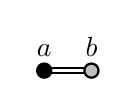
\begin{tikzpicture}[scale=.3]
    \draw (0,0.2) node[anchor=south] {$a$};
    \draw (2,0.2) node[anchor=south] {$b$};
    \foreach \x in {0}
    \draw[xshift=\x cm,thick,fill=black] (\x cm,0) circle (.3cm);
    \foreach \x in {1}
    \draw[xshift=\x cm,thick,fill=lightgray] (\x cm,0) circle (.3cm);
    \foreach \y in {0.15,...,0.15}
    \draw[xshift=\y cm,thick] (\y cm,+0.1 cm) -- +(1.4 cm,0);
    \foreach \y in {0.15,...,0.15}
    \draw[xshift=\y cm,thick] (\y cm,-0.1 cm) -- +(1.4 cm,0);
  \end{tikzpicture}
}

\newcommand{\DynkinBabc}{
  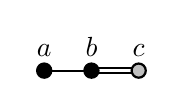
\begin{tikzpicture}[scale=.3]
    \draw (0,0.2) node[anchor=south] {$a$};
    \draw (2,0.2) node[anchor=south] {$b$};
    \draw (4,0.2) node[anchor=south] {$c$};
    \foreach \x in {0,1}
    \draw[xshift=\x cm,thick,fill=black] (\x cm,0) circle (.3cm);
    \foreach \x in {2}
    \draw[xshift=\x cm,thick,fill=lightgray] (\x cm,0) circle (.3cm);
    \foreach \y in {0.15,...,0.15}
    \draw[xshift=\y cm,thick] (\y cm,0) -- +(1.4 cm,0);
    \foreach \y in {1.15,...,1.15}
    \draw[xshift=\y cm,thick] (\y cm,+0.1 cm) -- +(1.4 cm,0);
    \foreach \y in {1.15,...,1.15}
    \draw[xshift=\y cm,thick] (\y cm,-0.1 cm) -- +(1.4 cm,0);
  \end{tikzpicture}
}


\newcommand{\DynkinCn}{
  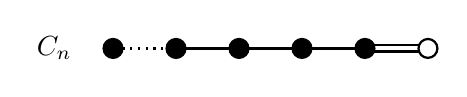
\begin{tikzpicture}[scale=.4]
    \draw (-1,0) node[anchor=east]  {$C_n$};
    \foreach \x in {0,...,4}
    \draw[xshift=\x cm,thick,fill=black] (\x cm,0) circle (.3cm);
    \draw[xshift=5 cm,thick] (5 cm, 0) circle (.3 cm);
    \draw[dotted,thick] (0.3 cm,0) -- +(1.4 cm,0);
    \foreach \y in {1.15,...,3.15}
    \draw[xshift=\y cm,thick] (\y cm,0) -- +(1.4 cm,0);
    \draw[thick] (8.3 cm, .1 cm) -- +(1.4 cm,0);
    \draw[thick] (8.3 cm, -.1 cm) -- +(1.4 cm,0);
  \end{tikzpicture}
}

\newcommand{\DynkinCab}{
  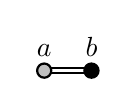
\begin{tikzpicture}[scale=.3]
    \draw (0,0.2) node[anchor=south] {$a$};
    \draw (2,0.2) node[anchor=south] {$b$};
    \foreach \x in {0}
    \draw[xshift=\x cm,thick,fill=lightgray] (\x cm,0) circle (.3cm);
    \foreach \x in {1}
    \draw[xshift=\x cm,thick,fill=black] (\x cm,0) circle (.3cm);
    \foreach \y in {0.15,...,0.15}
    \draw[xshift=\y cm,thick] (\y cm,+0.1 cm) -- +(1.4 cm,0);
    \foreach \y in {0.15,...,0.15}
    \draw[xshift=\y cm,thick] (\y cm,-0.1 cm) -- +(1.4 cm,0);
  \end{tikzpicture}
}

\newcommand{\DynkinCabc}{
  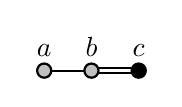
\begin{tikzpicture}[scale=.3]
    \draw (0,0.2) node[anchor=south] {$a$};
    \draw (2,0.2) node[anchor=south] {$b$};
    \draw (4,0.2) node[anchor=south] {$c$};
    \foreach \x in {0,1}
    \draw[xshift=\x cm,thick,fill=lightgray] (\x cm,0) circle (.3cm);
    \foreach \x in {2}
    \draw[xshift=\x cm,thick,fill=black] (\x cm,0) circle (.3cm);
    \foreach \y in {0.15,...,0.15}
    \draw[xshift=\y cm,thick] (\y cm,0) -- +(1.4 cm,0);
    \foreach \y in {1.15,...,1.15}
    \draw[xshift=\y cm,thick] (\y cm,+0.1 cm) -- +(1.4 cm,0);
    \foreach \y in {1.15,...,1.15}
    \draw[xshift=\y cm,thick] (\y cm,-0.1 cm) -- +(1.4 cm,0);
  \end{tikzpicture}
}


\newcommand{\DynkinDn}{
  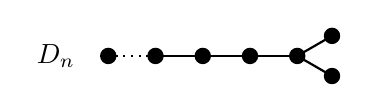
\begin{tikzpicture}[scale=.3]
    \draw (-1,0) node[anchor=east]  {$D_n$};
    \foreach \x in {0,...,4}
    \draw[xshift=\x cm,thick,fill=black] (\x cm,0) circle (.3cm);
    \draw[xshift=8 cm,thick,fill=black] (30: 17 mm) circle (.3cm);
    \draw[xshift=8 cm,thick,fill=black] (-30: 17 mm) circle (.3cm);
    \draw[dotted,thick] (0.3 cm,0) -- +(1.4 cm,0);
    \foreach \y in {1.15,...,3.15}
    \draw[xshift=\y cm,thick] (\y cm,0) -- +(1.4 cm,0);
    \draw[xshift=8 cm,thick] (30: 3 mm) -- (30: 14 mm);
    \draw[xshift=8 cm,thick] (-30: 3 mm) -- (-30: 14 mm);
  \end{tikzpicture}}

\newcommand{\DynkinGtwo}{
  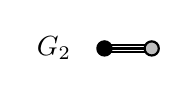
\begin{tikzpicture}[scale=.3]
    \draw (-1,0) node[anchor=east]  {$G_2$};
    \draw[thick,fill=black] (0 ,0) circle (.3 cm);
    \draw[thick,fill=lightgray] (2 cm,0) circle (.3 cm);
    \draw[thick] (30: 3mm) -- +(1.5 cm, 0);
    \draw[thick] (0: 3 mm) -- +(1.4 cm, 0);
    \draw[thick] (-30: 3 mm) -- +(1.5 cm, 0);
  \end{tikzpicture}}

\newcommand{\DynkinFfour}{
  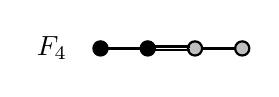
\begin{tikzpicture}[scale=.3]
    \draw (-3,0) node[anchor=east]  {$F_4$};
    \draw[thick,fill=black] (-2 cm ,0) circle (.3 cm);
    \draw[thick,fill=black] (0 ,0) circle (.3 cm);
    \draw[thick,fill=lightgray] (2 cm,0) circle (.3 cm);
    \draw[thick,fill=lightgray] (4 cm,0) circle (.3 cm);
    \draw[thick] (15: 3mm) -- +(1.5 cm, 0);
    \draw[xshift=-2 cm,thick] (0: 3 mm) -- +(1.4 cm, 0);
    \draw[thick] (-15: 3 mm) -- +(1.5 cm, 0);
    \draw[xshift=2 cm,thick] (0: 3 mm) -- +(1.4 cm, 0);
  \end{tikzpicture}}

\newcommand{\DynkinEsix}{
  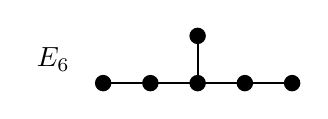
\begin{tikzpicture}[scale=.3]
    \draw (-1,1) node[anchor=east]  {$E_6$};
    \foreach \x in {0,...,4}
    \draw[thick,fill=black,xshift=\x cm] (\x cm,0) circle (3 mm);
    \foreach \y in {0,...,3}
    \draw[thick,xshift=\y cm] (\y cm,0) ++(.3 cm, 0) -- +(14 mm,0);
    \draw[thick,fill=black] (4 cm,2 cm) circle (3 mm);
    \draw[thick] (4 cm, 3mm) -- +(0, 1.4 cm);
  \end{tikzpicture}}

\newcommand{\DynkinEseven}{
  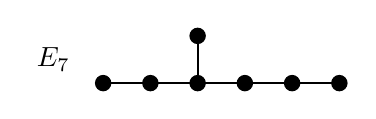
\begin{tikzpicture}[scale=.3]
    \draw (-1,1) node[anchor=east]  {$E_7$};
    \foreach \x in {0,...,5}
    \draw[thick,fill=black,xshift=\x cm] (\x cm,0) circle (3 mm);
    \foreach \y in {0,...,4}
    \draw[thick,xshift=\y cm] (\y cm,0) ++(.3 cm, 0) -- +(14 mm,0);
    \draw[thick,fill=black] (4 cm,2 cm) circle (3 mm);
    \draw[thick] (4 cm, 3mm) -- +(0, 1.4 cm);
  \end{tikzpicture}}

\newcommand{\DynkinEeight}{
  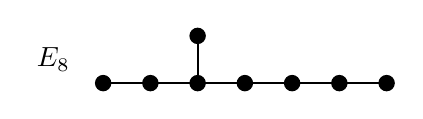
\begin{tikzpicture}[scale=.3]
    \draw (-1,1) node[anchor=east]  {$E_8$};
    \foreach \x in {0,...,6}
    \draw[thick,fill=black,xshift=\x cm] (\x cm,0) circle (3 mm);
    \foreach \y in {0,...,5}
    \draw[thick,xshift=\y cm] (\y cm,0) ++(.3 cm, 0) -- +(14 mm,0);
    \draw[thick,fill=black] (4 cm,2 cm) circle (3 mm);
    \draw[thick] (4 cm, 3mm) -- +(0, 1.4 cm);
  \end{tikzpicture}}




%\title{The philosophy of cusp forms?}
\title{Parabolic Induction}

%\author{Sijato Budotr}
\author{Simon Burton}

\date{\today}

\flushbottom

\begin{document}

\maketitle

We are trying to make sense of the ``philosophy of cusp forms''
which is explained in chapter 47 of \cite{Bump2004},
and also the categorified representation rings of \cite{Joyal1995}.
Part of this is the correspondence (duality)
between the irreducible complex
representations of a group $G$ and the 
conjugacy classes of the Langlands dual group $G^{\vee}$.

\section{$\GL(n,\Field_q)$}

Recall the $q$-deformed Pascal triangle, for $q=2$ this begins:
$$
\begin{tikzcd}[column sep=small, row sep=small]
 &  &  &  &  &  &  & 1\arrow[dl, swap, "2^0"]\arrow[dr] &  &  &  &  &  \\
A_0: &  &  &  &  &  & 1\arrow[dl, swap, "2^{0}"]\arrow[dr] &  & 1\arrow[dl, swap, "2^{1}"]\arrow[dr] &  &  &  &  \\
A_1: &  &  &  &  & 1\arrow[dl, swap, "2^{0}"]\arrow[dr] &  & 3\arrow[dl, swap, "2^{1}"]\arrow[dr] &  & 1\arrow[dl, swap, "2^{2}"]\arrow[dr] &  &  &  \\
A_2: &  &  &  & 1\arrow[dl, swap, "2^{0}"]\arrow[dr] &  & 7\arrow[dl, swap, "2^{1}"]\arrow[dr] &  & 7\arrow[dl, swap, "2^{2}"]\arrow[dr] &  & 1\arrow[dl, swap, "2^{3}"]\arrow[dr] &  &  \\
A_3: &  &  & 1\arrow[dl, swap, "2^{0}"]\arrow[dr] &  & 15\arrow[dl, swap, "2^{1}"]\arrow[dr] &  & 35\arrow[dl, swap, "2^{2}"]\arrow[dr] &  & 15\arrow[dl, swap, "2^{3}"]\arrow[dr] &  & 1\arrow[dl, swap, "2^{4}"]\arrow[dr] &  \\
A_4: &  & 1 &  & 31 &  & 155 &  & 155 &  & 31 &  & 1 \\
\end{tikzcd}
$$
which is sequence A022166 in the OEIS.

Elements of a 
conjugacy class of $\GL(n,\Field_q)$ have the same characteristic polynomial.
In the tables below, for each conjugacy class,
we notate a representative matrix (or matrices) together with its
characteristic polynomial, the corresponding complex irrep,
and the dimension of the irrep.
Cuspidal irreps are given names $A, B, C,$ etc.
These are combined using the monoidal product
$\tensor$ and Schur functors.
So far, much of this is numerological guesswork and should not be particularly trusted.

%$$
%\begin{array}{cc}
%\end{array}
%$$

\setlength{\tabcolsep}{10pt}
\setlength{\arraycolsep}{1pt}
\renewcommand{\arraystretch}{0.5}

%\begin{center}
%\begin{tabular}{c|c}
%\# & char. poly \\
%\hline
%1 & $(x+1)^3$ \\
%21 & $(x+1)^3$ \\
%24 & $x^3+x^2+1$ \\
%24 & $x^3+x+1$ \\
%42 & $(x+1)^3$ \\
%56 & $(x+1)(x^2+x+1)$ \\
%\end{tabular}
%\end{center}

$G=\GL(1,\Field_2)$ has order 1, with 1 conjugacy class:
\begin{center}
\begin{tabular}{r|l|c|c|c}
\# & representative & char. polynomial & irrep & dim. \\
\hline
1 & $[1]$           & $x+1$            & $A$   & 1    \\
\end{tabular}
\end{center}

$G=\GL(2,\Field_2) \cong S_3$ has order 6, with 3 conjugacy classes:
\begin{center}
\begin{tabular}{r|l|c|c|c}
\# & representative(s) & char. polynomial & irrep & dim. \\
\hline
1  & $\begin{bmatrix}1&.\\.&1\end{bmatrix}$    & $(x+1)^2$  & $\yng(2)(A)$  & 1 \\
2  & $\begin{bmatrix}.&1\\1&1\end{bmatrix}$     & $x^2+x+1$  &  $B$  & 1 \\
3  & $\begin{bmatrix}1&1\\.&1\end{bmatrix}$    & $(x+1)^2$  & $\yng(1,1)(A)$ & 2  \\
\end{tabular}
\end{center}

$G=\GL(3,\Field_2)$ has order 168 and 6 conjugacy classes:
\begin{center}
\begin{tabular}{r|l|c|c|c}
\# & representative(s) & char. polynomial & irrep & dim. \\
\hline
 1 & $\begin{bmatrix}1&.&.\\.&1&.\\.&.&1\end{bmatrix}$ & $(x+1)^3$  
    & $\yng(3)(A)$ & 1 \\
21 & $\begin{bmatrix}1&1&.\\.&1&.\\.&.&1\end{bmatrix}$ ,
     $\begin{bmatrix}1&.&.\\.&1&1\\.&.&1\end{bmatrix}$ & $(x+1)^3$  
    & $\yng(1,2)(A)$ & 6  \\
24 & 
$\begin{bmatrix}1&1&.\\1&.&1\\.&1&.\end{bmatrix}$
,
$\begin{bmatrix}.&1&.\\1&.&1\\.&1&1\end{bmatrix}$
& $x^3+x^2+1$      & $C$ & 3 \\
24 & 
$\begin{bmatrix}1&1&.\\1&1&1\\.&1&.\end{bmatrix}$
,
$\begin{bmatrix}.&1&.\\1&1&1\\.&1&1\end{bmatrix}$
& $x^3+x+1$        & $C^{\star}$ & 3 \\
42 & $\begin{bmatrix}1&1&1\\.&1&1\\.&.&1\end{bmatrix}$
    ,  $\begin{bmatrix}1&1&.\\.&1&1\\.&.&1\end{bmatrix}$
    & $(x+1)^3$ 
    & $\yng(1,1,1)(A)$ & 8  \\
56 & $\begin{bmatrix}1&.&.\\.&1&1\\.&1&.\end{bmatrix}$ & $(x+1)(x^2+x+1)$
    & $A\tensor B$ & 7 \\
\hline
\strut =168 \\
\end{tabular}
\end{center}


$G=\GL(4,\Field_2)\cong A_8$ has order 20160 and 14 conjugacy classes:
\begin{center}
\begin{tabular}{r|l|c|c|c}
\# & representative & char. polynomial & irrep & dim. \\
\hline
1  & $\begin{bmatrix}1&.&.&.\\.&1&.&.\\.&.&1&.\\.&.&.&1\end{bmatrix}$  & $(x+1)^4$  & $\yng(4)(A)$ & 1  \\
105  & $\begin{bmatrix}1&1&.&.\\.&1&.&.\\.&.&1&.\\.&.&.&1\end{bmatrix}$  & $(x+1)^4$  & $\yng(1,3)(A)$ & 14?  \\
112  & $\begin{bmatrix}1&1&.&.\\1&.&.&.\\.&.&1&1\\.&.&1&.\end{bmatrix}$  & $(x^2+x+1)^2$  & $\yng(2)(B)$ & 7  \\
210  & $\begin{bmatrix}1&1&.&.\\.&1&.&.\\.&.&1&1\\.&.&.&1\end{bmatrix}$  & $(x+1)^4$  & $\yng(2,2)(A)$ & 20?  \\
1120  & $\begin{bmatrix}1&.&.&.\\.&1&.&.\\.&.&1&1\\.&.&1&.\end{bmatrix}$
  & $(x+1)^2(x^2+x+1)$  & $\yng(2)(A)\tensor B$ & 35  \\
1260  & $\begin{bmatrix}1&1&.&.\\.&1&1&.\\.&.&1&.\\.&.&.&1\end{bmatrix}$  & $(x+1)^4$  & $\yng(1,1,2)(A)$ & 56?  \\
1344  & 
$\begin{bmatrix}.&1&.&.\\1&1&1&.\\.&1&.&1\\.&.&1&.\end{bmatrix}$,
$\begin{bmatrix}.&1&.&.\\1&.&1&.\\.&1&1&1\\.&.&1&.\end{bmatrix}$
& $x^4+x^3+x^2+x+1$  & $D$ & 21  \\
1344  & 
$\begin{bmatrix}1&1&.&.\\1&1&1&.\\.&1&.&1\\.&.&1&1\end{bmatrix}$,
$\begin{bmatrix}1&1&.&.\\1&.&1&.\\.&1&1&1\\.&.&1&1\end{bmatrix}$
& $x^4+x^3+1$        & $E$ & 21  \\
1344  & 
$\begin{bmatrix}.&1&.&.\\1&1&1&.\\.&1&.&1\\.&.&1&1\end{bmatrix}$,
$\begin{bmatrix}1&1&.&.\\1&.&1&.\\.&1&1&1\\.&.&1&.\end{bmatrix}$
& $x^4+x+1$          & $E^\star$ & 21  \\
1680  & $\begin{bmatrix}1&1&1&1\\1&.&1&.\\.&.&1&1\\.&.&1&.\end{bmatrix}$  & $(x^2+x+1)^2$  & $\yng(1,1)(B)$ & 28  \\
2520  & $\begin{bmatrix}1&1&.&.\\.&1&1&.\\.&.&1&1\\.&.&.&1\end{bmatrix}$  & $(x+1)^4$  & $\yng(1,1,1,1)(A)$ & 64   \\
2880  & $\begin{bmatrix}1&.&.&.\\.&1&1&.\\.&1&.&1\\.&.&1&.\end{bmatrix}$
  & $(x+1)(x^3+x^2+1)$  & $A\tensor C$ & 45   \\
2880  & $\begin{bmatrix}1&.&.&.\\.&1&1&.\\.&1&1&1\\.&.&1&.\end{bmatrix}$
  & $(x+1)(x^3+x+1)$  & $A\tensor C^{\star}$ & 45   \\
3360  & $\begin{bmatrix}1&1&.&.\\.&1&.&.\\.&.&1&1\\.&.&1&.\end{bmatrix}$  & $(x+1)^2(x^2+x+1)$  & $\yng(1,1)(A)\tensor B$ & 70 \\
\hline
\strut = 20160 \\
\end{tabular}
\end{center}
Where the irrep dimensions have square sum:
$$
 20160 = 1^2 + 7^2 + 14^2 + 20^2 + 21^2 + 21^2 + 21^2 + 28^2 + 35^2 + 45^2 + 45^2 + 56^2 + 64^2 + 70^2.
$$


$G=\GL(5,\Field_2)$ has order 9999360 and 27 conjugacy classes/irreps:
$$
\begin{array}{ccccr}
    &             \text{char. polynomial}  &  \text{factored} & \text{irrep} & \text{dim.}  \\
\hline
    &               x^5+x^4+x+1 &                 (x+1)^5 & \yng(5)(A)                   &  1  \\
    &               x^5+x^4+x+1 &                 (x+1)^5 & \yng(4,1)(A)                 &  2\times 15=30  \\
    &               x^5+x^4+x+1 &                 (x+1)^5 & \yng(3,2)(A)                 &  4\times 31=124  \\
    &               x^5+x^4+x+1 &                 (x+1)^5 & \yng(3,1,1)(A)               &  8\times 35=280  \\
    &               x^5+x^4+x+1 &                 (x+1)^5 & \yng(2,2,1)(A)               &  16\times 31=496  \\
    &               x^5+x^4+x+1 &                 (x+1)^5 & \yng(2,1,1,1)(A)             &  64\times 15=960  \\
    &               x^5+x^4+x+1 &                 (x+1)^5 & \yng(1,1,1,1,1)(A)           &  1024  \\
    &             x^5+x^3+x^2+1 &       (x+1)^3(x^2+x+1)  & \yng(3)(A)\tensor B      &  155   \\
    &             x^5+x^3+x^2+1 &       (x+1)^3(x^2+x+1)  & \yng(2,1)(A)\tensor B        &  6\times 155=930   \\
    &             x^5+x^3+x^2+1 &       (x+1)^3(x^2+x+1)  & \yng(1,1,1)(A)\tensor B          &  \hsp 8\times 155=1240   \\
    &       x^5+x^4+x^3+x^2+x+1 &       (x+1)(x^2+x+1)^2  & A\tensor\yng(2)(B)         &  7 \times 31 = 217  \\
    &       x^5+x^4+x^3+x^2+x+1 &       (x+1)(x^2+x+1)^2  & A\tensor \yng(1,1)(B)          &  28 \times 31 = 868  \\
    &             x^5+x^4+x^3+1 &     (x+1)^2(x^3+x^2+1)  & \yng(2)(A)\tensor C        &  1 \times 3 \times 155=465   \\
    &             x^5+x^4+x^3+1 &     (x+1)^2(x^3+x^2+1)  & \yng(1,1)(A)\tensor C          &  2 \times 3 \times 155=930  \\
    &               x^5+x^2+x+1 &       (x+1)^2(x^3+x+1)  & \yng(2)(A)\tensor C^{\star}&  1 \times 3 \times 155=465   \\
    &               x^5+x^2+x+1 &       (x+1)^2(x^3+x+1)  & \yng(1,1)(A)\tensor C^{\star}  &  2 \times 3 \times 155=930   \\
    &               x^5+x^3+x+1 &       (x+1)(x^4+x^3+1)  & A\tensor E                   &  21\times 31=651   \\
    &             x^5+x^4+x^2+1 &         (x+1)(x^4+x+1)  & A\tensor E^{\star}           &  21\times 31=651   \\
    &                   x^5+x+1 &   (x^2+x+1)(x^3+x^2+1)  & B\tensor C                   &  3\times 155=465   \\
    &                 x^5+x^4+1 &     (x^2+x+1)(x^3+x+1)  & B\tensor C^{\star}           &  3\times 155=465   \\
    &                     x^5+1 & (x+1)(x^4+x^3+x^2+x+1)  & A\tensor D                   &  21\times 31=651   \\
    &         x^5+x^4+x^3+x^2+1 &       x^5+x^4+x^3+x^2+1 & F                            & 315   \\
    &           x^5+x^3+x^2+x+1 &         x^5+x^3+x^2+x+1 & F^{\star}                    & 315   \\
    &           x^5+x^4+x^3+x+1 &         x^5+x^4+x^3+x+1 & G                            & 315   \\
    &           x^5+x^4+x^2+x+1 &         x^5+x^4+x^2+x+1 & G^{\star}                    & 315   \\
    &                 x^5+x^3+1 &               x^5+x^3+1 & H                            & 315   \\
    &                 x^5+x^2+1 &               x^5+x^2+1 & H^{\star}                    & 315   \\
\end{array}
$$
%Leftovers: 
%$
%30=2.3.5, 124=2^2.31, 280=2^3.5.7, 496=2^4.31, 960=2^6.3.5.
%$

The dimensions of the irreps are:
$
1, 30, 124, 155, 217,
280, 
315, 315, 315, 315, 315, 315,\\
465, 465, 
465, 465, 
496, 
651, 651, 651, 868, 
930, 930, 930, 
960, 1024, 1240.
$

We tabulate how many times the characteristic polynomial $(x+1)^n$ appears
in the conjugacy classes of $\GL(n,\Field_2)$:
\begin{center}\begin{tabular}{c|r|r}
$\GL(n,\Field_2)$ & cgy. classes  & \# $(x+1)^n$ \\
\hline
$\GL(1,\Field_2)$  & 1    & 1 \\
$\GL(2,\Field_2)$  & 3    & 2 \\
$\GL(3,\Field_2)$  & 6   & 3 \\
$\GL(4,\Field_2)$  & 14   & 5 \\
$\GL(5,\Field_2)$  & 27   & 7 \\
$\GL(6,\Field_2)$  & 60   & 11 \\
$\GL(7,\Field_2)$  & 117   & 15 \\
\end{tabular} \end{center}
Evidently these numbers 1,2,3,5,.. count the partitions on $n$.


The dimension of the cuspidal representations is given by the $q$-polynomials
$
1, q-1=1, 
(q^2-1)(q-1)=3, 
(q^3-1)(q^2-1)(q-1)=21, 
(q^4-1)(q^3-1)(q^2-1)(q-1)=315, ...
$


\section{$\GL(n,\Field_3)$}

$G=\GL(1,\Field_3)$ has order 2, with 2 conjugacy class:
\begin{center}
\begin{tabular}{r|l|c|c|c}
\# & representative & char. polynomial & irrep & dim. \\
\hline
1 & $[2]$           & $x+1$            & $A$   & 1    \\
1 & $[1]$           & $x+2$            & $B$   & 1    \\
\end{tabular}
\end{center}

$|\GL(2,\Field_3)|=48$

%|G| = 48
%inv:[0]
%char classes: 8
%[1, 1, 6, 6, 6, 8, 8, 12] == 48

%[ Character( CharacterTable( GL(2,3) ), [ 1, 1, 1, 1, 1, 1, 1, 1 ] ),
%  Character( CharacterTable( GL(2,3) ), [ 1, 1, 1, 1, 1, -1, -1, -1 ] ),
%  Character( CharacterTable( GL(2,3) ), [ 2, -1, 2, -1, 2, 0, 0, 0 ] ),
%  Character( CharacterTable( GL(2,3) ), [ 2, 1, -2, -1, 0, -E(8)-E(8)^3, E(8)+E(8)^3, 0 ] ),
%  Character( CharacterTable( GL(2,3) ), [ 2, 1, -2, -1, 0, E(8)+E(8)^3, -E(8)-E(8)^3, 0 ] ),
%  Character( CharacterTable( GL(2,3) ), [ 3, 0, 3, 0, -1, 1, 1, -1 ] ),
%  Character( CharacterTable( GL(2,3) ), [ 3, 0, 3, 0, -1, -1, -1, 1 ] ),
%  Character( CharacterTable( GL(2,3) ), [ 4, -1, -4, 1, 0, 0, 0, 0 ] ) ]

\begin{center}
\begin{tabular}{r|l|c|c|c}
\# & representative & char. polynomial & irrep & dim. \\
\hline
1  &  $\begin{bmatrix}2&.\\.&2\end{bmatrix}$   & $(x+1)^2$  & $\yng(2)(A)$ & 1  \\
1  &  $\begin{bmatrix}1&.\\.&1\end{bmatrix}$   & $(x+2)^2$  & $\yng(2)(B)$ & 1  \\
6  &  $\begin{bmatrix}.&1\\1&1\end{bmatrix}$   & $x^2+2x+2$  & $C$ & 2  \\
6  &  $\begin{bmatrix}.&1\\1&2\end{bmatrix}$   & $x^2+x+2$  & $C^\star$ & 2  \\
6  &  $\begin{bmatrix}.&2\\1&.\end{bmatrix}$   & $x^2+1$  & $D$ & 2  \\
8  &  $\begin{bmatrix}2&1\\.&2\end{bmatrix}$   & $(x+1)^2$  & $\yng(1,1)(A)$ & 3  \\
8  &  $\begin{bmatrix}1&1\\.&1\end{bmatrix}$   & $(x+2)^2$  & $\yng(1,1)(B)$ & 3  \\
12  &  $\begin{bmatrix}2&.\\.&1\end{bmatrix}$   & $(x+1)(x+2)$  & $A\tensor B$ & 4  \\
\end{tabular}
\end{center}


\section{$\GL(n,\Field_5)$}


$\GL(1,\Field_5)$

$$
\begin{array}{c|c|c|c|r}
\#    &             \text{representative}  &  \text{factored} & \text{irrep} & \text{dim.}  \\
\hline
1  &  \begin{bmatrix}4\end{bmatrix}   & x+1  & A & 1  \\
1  &  \begin{bmatrix}3\end{bmatrix}   & x+2  & B & 1  \\
1  &  \begin{bmatrix}2\end{bmatrix}   & x+3  & C & 1  \\
1  &  \begin{bmatrix}1\end{bmatrix}   & x+4  & D & 1  \\
\end{array}
$$

$\GL(2,\Field_5)$

%[ 1, 1, 1, 1, 1, 1, 1, 1, 1, 1, 1, 1, 1, 1, 1, 1, 1, 1, 1, 1, 1, 1, 1, 1 ] ), 
%[ 1, 1, 1, 1, 1, 1, 1, 1, 1, 1, -1, -1, -1, 1, 1, -1, -1, -1, -1, 1, -1, -1, 1, -1 ] ), 
%[ 1, 1, -1, -1, 1, 1, -1, -1, 1, 1, -E(4), -E(4), -E(4), -1, -1, E(4), E(4), E(4), -E(4), -1, E(4), E(4), 1, -E(4) ] ), 
%[ 1, 1, -1, -1, 1, 1, -1, -1, 1, 1, E(4), E(4), E(4), -1, -1, -E(4), -E(4), -E(4), E(4), -1, -E(4), -E(4), 1, E(4) ] ), 
%[ 4, -1, 4, -1, 4, -1, 4, -1, 1, 1, -2, 1, 1, 1, 1, -2, 1, 1, 0, 0, 0, 0, 0, 0 ] ), 
%[ 4, -1, 4, -1, 4, -1, 4, -1, 1, 1, 2, -1, -1, 1, 1, 2, -1, -1, 0, 0, 0, 0, 0, 0 ] ), 
%[ 4, 1, 4*E(4), -E(4), -4, -1, -4*E(4), E(4), -2, 2, 0, 0, 0, 2*E(4), -2*E(4), 0, 0, 0, 0, 0, 0, 0, 0, 0 ] ), 
%[ 4, 1, -4*E(4), E(4), -4, -1, 4*E(4), -E(4), -2, 2, 0, 0, 0, -2*E(4), 2*E(4), 0, 0, 0, 0, 0, 0, 0, 0, 0 ] ), 
%[ 4, -1, -4, 1, 4, -1, -4, 1, 1, 1, 2*E(4), -E(4), -E(4), -1, -1, -2*E(4), E(4), E(4), 0, 0, 0, 0, 0, 0 ] ), 
%[ 4, -1, -4, 1, 4, -1, -4, 1, 1, 1, -2*E(4), E(4), E(4), -1, -1, 2*E(4), -E(4), -E(4), 0, 0, 0, 0, 0, 0 ] ), 
%[ 4, 1, 4*E(4), -E(4), -4, -1, -4*E(4), E(4), 1, -1, 0, E(24)^11-E(24)^19, -E(24)^11+E(24)^19, -E(4), E(4), 0, E(24)-E(24)^17, -E(24)+E(24)^17, 0, 0, 0, 0, 0, 0 ] ), 
%[ 4, 1, 4*E(4), -E(4), -4, -1, -4*E(4), E(4), 1, -1, 0, -E(24)^11+E(24)^19, E(24)^11-E(24)^19, -E(4), E(4), 0, -E(24)+E(24)^17, E(24)-E(24)^17, 0, 0, 0, 0, 0, 0 ] ), 
%[ 4, 1, -4*E(4), E(4), -4, -1, 4*E(4), -E(4), 1, -1, 0, E(24)-E(24)^17, -E(24)+E(24)^17, E(4), -E(4), 0, E(24)^11-E(24)^19, -E(24)^11+E(24)^19, 0, 0, 0, 0, 0, 0 ] ), 
%[ 4, 1, -4*E(4), E(4), -4, -1, 4*E(4), -E(4), 1, -1, 0, -E(24)+E(24)^17, E(24)-E(24)^17, E(4), -E(4), 0, -E(24)^11+E(24)^19, E(24)^11-E(24)^19, 0, 0, 0, 0, 0, 0 ] ), 
%[ 5, 0, 5, 0, 5, 0, 5, 0, -1, -1, 1, 1, 1, -1, -1, 1, 1, 1, -1, 1, -1, -1, 1, -1 ] ), 
%[ 5, 0, 5, 0, 5, 0, 5, 0, -1, -1, -1, -1, -1, -1, -1, -1, -1, -1, 1, 1, 1, 1, 1, 1 ] ), 
%[ 5, 0, -5, 0, 5, 0, -5, 0, -1, -1, E(4), E(4), E(4), 1, 1, -E(4), -E(4), -E(4), -E(4), -1, E(4), E(4), 1, -E(4) ] ), 
%[ 5, 0, -5, 0, 5, 0, -5, 0, -1, -1, -E(4), -E(4), -E(4), 1, 1, E(4), E(4), E(4), E(4), -1, -E(4), -E(4), 1, E(4) ] ), 
%[ 6, 1, 6, 1, 6, 1, 6, 1, 0, 0, 0, 0, 0, 0, 0, 0, 0, 0, 0, -2, 0, 0, -2, 0 ] ), 
%[ 6, 1, -6, -1, 6, 1, -6, -1, 0, 0, 0, 0, 0, 0, 0, 0, 0, 0, 0, 2, 0, 0, -2, 0 ] ), 
%[ 6, -1, -6*E(4), -E(4), -6, 1, 6*E(4), E(4), 0, 0, 0, 0, 0, 0, 0, 0, 0, 0, 1+E(4), 0, 1-E(4), -1+E(4), 0, -1-E(4) ] ), 
%[ 6, -1, 6*E(4), E(4), -6, 1, -6*E(4), -E(4), 0, 0, 0, 0, 0, 0, 0, 0, 0, 0, 1-E(4), 0, 1+E(4), -1-E(4), 0, -1+E(4) ] ), 
%[ 6, -1, 6*E(4), E(4), -6, 1, -6*E(4), -E(4), 0, 0, 0, 0, 0, 0, 0, 0, 0, 0, -1+E(4), 0, -1-E(4), 1+E(4), 0, 1-E(4) ] ), 
%[ 6, -1, -6*E(4), -E(4), -6, 1, 6*E(4), E(4), 0, 0, 0, 0, 0, 0, 0, 0, 0, 0, -1-E(4), 0, -1+E(4), 1-E(4), 0, 1+E(4) ] ) ]


Here we label the new cuspidals $E$ through $N$, even though we don't know
the exact order these appear in, ie.
the exact correspondence
between the cuspidals $E-N$ and the conjugacy classes of $\GL(2,\Field_5)$ is unknown.
$$
\begin{array}{c|c|c|c|r}
\#    &             \text{representative}  &  \text{factored} & \text{irrep} & \text{dim.}  \\
\hline
1  &  \begin{bmatrix}4&.\\.&4\end{bmatrix}   & (x+1)^2  & \yng(2)(A) & 1  \\
1  &  \begin{bmatrix}3&.\\.&3\end{bmatrix}   & (x+2)^2  & \yng(2)(B) & 1  \\
1  &  \begin{bmatrix}2&.\\.&2\end{bmatrix}   & (x+3)^2  & \yng(2)(C) & 1  \\
1  &  \begin{bmatrix}1&.\\.&1\end{bmatrix}   & (x+4)^2  & \yng(2)(D) & 1  \\
20  &  \begin{bmatrix}.&3\\1&1\end{bmatrix}   & x^2+4x+2  & E & 4  \\
20  &  \begin{bmatrix}.&2\\1&.\end{bmatrix}   & x^2+3     & F & 4  \\
20  &  \begin{bmatrix}.&3\\1&.\end{bmatrix}   & x^2+2     & G & 4  \\
20  &  \begin{bmatrix}.&2\\1&2\end{bmatrix}   & x^2+3x+3  & H & 4  \\
20  &  \begin{bmatrix}.&4\\1&1\end{bmatrix}   & x^2+4x+1  & I & 4  \\
20  &  \begin{bmatrix}.&1\\1&3\end{bmatrix}   & x^2+2x+4  & J & 4  \\
20  &  \begin{bmatrix}.&2\\1&3\end{bmatrix}   & x^2+2x+3  & K & 4  \\
20  &  \begin{bmatrix}.&1\\1&2\end{bmatrix}   & x^2+3x+4  & L & 4  \\
20  &  \begin{bmatrix}.&4\\1&4\end{bmatrix}   & x^2+x+1   & M & 4  \\
20  &  \begin{bmatrix}.&3\\1&4\end{bmatrix}   & x^2+x+2   & N & 4  \\
24  &  \begin{bmatrix}.&4\\1&3\end{bmatrix}   & (x+1)^2   & \yng(1,1)(A) & 5  \\
24  &  \begin{bmatrix}.&1\\1&1\end{bmatrix}   & (x+2)^2   & \yng(1,1)(B) & 5  \\
24  &  \begin{bmatrix}.&1\\1&4\end{bmatrix}   & (x+3)^2   & \yng(1,1)(C) & 5  \\
24  &  \begin{bmatrix}.&4\\1&2\end{bmatrix}   & (x+4)^2   & \yng(1,1)(D) & 5  \\
30  &  \begin{bmatrix}.&3\\1&2\end{bmatrix}   & (x+1)(x+2)  & A\tensor B & 6  \\
30  &  \begin{bmatrix}.&2\\1&1\end{bmatrix}   & (x+1)(x+3)  & A\tensor C & 6  \\
30  &  \begin{bmatrix}.&1\\1&.\end{bmatrix}   & (x+1)(x+4)  & A\tensor D & 6  \\
30  &  \begin{bmatrix}.&4\\1&.\end{bmatrix}   & (x+2)(x+3)  & B\tensor C & 6  \\
30  &  \begin{bmatrix}.&2\\1&4\end{bmatrix}   & (x+2)(x+4)  & B\tensor D & 6  \\
30  &  \begin{bmatrix}.&3\\1&3\end{bmatrix}   & (x+3)(x+4)  & C\tensor D & 6  \\
\end{array}
$$

We choose a torus subgroup $T$ of $\GL(2,\Field_5)$ of order 24.
Then we induce characters of $T$ up to $\GL(2,\Field_5)$ and show the
irreducible content of these induced representations.
The blue lines denote orbits of the Frobenius in $\GL(1,\Field_{25})$.

\begin{center}
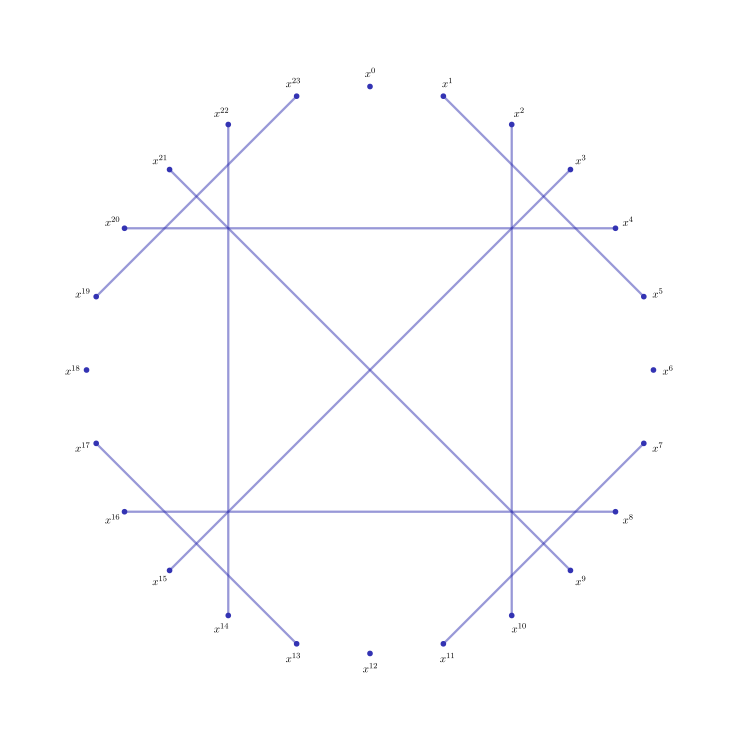
\includegraphics[scale=0.5]{images/cusp_24.pdf}
\end{center}

%\begin{center}
%\begin{tabular}{r|l|c|c|c}
%\# & representative & char. polynomial & irrep & dim. \\
%\hline
%1  &   & $(x+1)^2$  & ? & ?  \\
%1  &   & $(x+3)^2$  & ? & ?  \\
%1  &   & $(x+2)^2$  & ? & ?  \\
%1  &   & $(x+4)^2$  & ? & ?  \\
%20  &   & $x^2+4x+2$  & ? & ?  \\
%20  &   & $x^2+2x+4$  & ? & ?  \\
%20  &   & $x^2+4x+1$  & ? & ?  \\
%20  &   & $x^2+3x+4$  & ? & ?  \\
%20  &   & $x^2+2$  & ? & ?  \\
%20  &   & $x^2+x+1$  & ? & ?  \\
%20  &   & $x^2+3$  & ? & ?  \\
%20  &   & $x^2+2x+3$  & ? & ?  \\
%20  &   & $x^2+3x+3$  & ? & ?  \\
%20  &   & $x^2+x+2$  & ? & ?  \\
%24  &   & $(x+3)^2$  & ? & ?  \\
%24  &   & $(x+1)^2$  & ? & ?  \\
%24  &   & $(x+4)^2$  & ? & ?  \\
%24  &   & $(x+2)^2$  & ? & ?  \\
%30  &   & $(x+1)(x+3)$  & ? & ?  \\
%30  &   & $(x+1)(x+2)$  & ? & ?  \\
%30  &   & $(x+2)(x+3)$  & ? & ?  \\
%30  &   & $(x+3)(x+4)$  & ? & ?  \\
%30  &   & $(x+1)(x+4)$  & ? & ?  \\
%30  &   & $(x+2)(x+4)$  & ? & ?  \\
%\end{tabular}
%\end{center}
%




\section{$\Sp(2n,\Field_q)$}

%See also:
%``Classification of the Subgroups of the Two-Qubit Clifford Group''
%    Eric Kubischta, Ian Teixeira
% https://arxiv.org/abs/2409.14624
% 

Note that $\Sp(2n,\Field_2) \cong \SO(2n+1,\Field_2)$.

$G=\Sp(2,\Field_2)\cong \GL(2,\Field_2)$ as above.

$G=\Sp(4,\Field_2)\cong S_6$ has order 720 and 11 conjugacy classes:
\begin{center}
\begin{tabular}{r|l|c|c|c}
\# & representative & char. polynomial & irrep & dim. \\
\hline
1  & $\begin{bmatrix}1&.&.&.\\.&1&.&.\\.&.&1&.\\.&.&.&1\end{bmatrix}$  & $(x+1)^4$  & ? & 1  \\
15  & $\begin{bmatrix}1&.&.&.\\.&1&.&1\\1&.&1&.\\.&.&.&1\end{bmatrix}=CX_{0,1}$
    & $(x+1)^4$  & ? & ?  \\
15  & $\begin{bmatrix}1&1&.&.\\.&1&.&.\\.&.&1&.\\.&.&.&1\end{bmatrix}$  & $(x+1)^4$  & ? & ?  \\
40  &  $\begin{bmatrix}1&.&.&.\\.&1&.&.\\.&.&1&1\\.&.&1&.\end{bmatrix}$   & $(x+1)^2(x^2+x+1)$  & ? & ?  \\
40  & $\begin{bmatrix}1&1&.&.\\1&.&.&.\\.&.&1&1\\.&.&1&.\end{bmatrix}$    & $(x^2+x+1)^2$  & ? & ?  \\
45  & $\begin{bmatrix}1&1&.&.\\.&1&.&.\\.&.&1&1\\.&.&.&1\end{bmatrix}$  & $(x+1)^4$  & ? & ?  \\
90  &  $\begin{bmatrix}.&.&.&.\\.&.&.&.\\.&.&.&.\\.&.&.&.\end{bmatrix}$ ?  & $(x+1)^4$  & ? & ?  \\
90  & $\begin{bmatrix}.&.&.&.\\.&.&.&.\\.&.&.&.\\.&.&.&.\end{bmatrix}$  ?  & $(x+1)^4$  & ? & ?  \\
120  & $\begin{bmatrix}.&.&.&.\\.&.&.&.\\.&.&.&.\\.&.&.&.\end{bmatrix}$ ?   & $(x^2+x+1)^2$  & ? & ?  \\
120  & $\begin{bmatrix}1&1&.&.\\.&1&.&.\\.&.&1&1\\.&.&1&.\end{bmatrix}$     & $(x+1)^2(x^2+x+1)$  & ? & ?  \\
144  & $\begin{bmatrix}.&1&.&.\\1&1&1&.\\.&1&.&1\\.&.&1&.\end{bmatrix}$    & $x^4+x^3+x^2+x+1$  & $D$ & ?  \\
\hline
\strut = 720 \\
\end{tabular}
\end{center}
The irreps have dimension: 1, 1, 5, 5, 5, 5, 9, 9, 10, 10, 16.
% https://beta.lmfdb.org/Groups/Abstract/720.763

$G = \Sp(6,\Field_2)$  has order 1451520 and 30 conjugacy classes:

\begin{center}
\begin{tabular}{r|l|c|c|c}
\# & representative & char. polynomial & irrep & dim. \\
\hline
1  & & $(x+1)^6$  & ? & ?  \\
63  & & $(x+1)^6$  & ? & ?  \\
315  & & $(x+1)^6$  & ? & ?  \\
672  & & $(x+1)^4(x^2+x+1)$  & ? & ?  \\
945  & & $(x+1)^6$  & ? & ?  \\
2240  & & $(x^2+x+1)^3$  & ? & ?  \\
3780  & & $(x+1)^6$  & ? & ?  \\
3780  & & $(x+1)^6$  & ? & ?  \\
7560  & & $(x+1)^6$  & ? & ?  \\
7560  & & $(x+1)^6$  & ? & ?  \\
10080  & & $(x+1)^4(x^2+x+1)$  & ? & ?  \\
10080  & & $(x+1)^4(x^2+x+1)$  & ? & ?  \\
11340  & & $(x+1)^6$  & ? & ?  \\
13440  & & $(x+1)^2(x^2+x+1)^2$  & ? & ?  \\
20160  & & $(x^2+x+1)^3$  & ? & ?  \\
30240  & & $(x+1)^4(x^2+x+1)$  & ? & ?  \\
40320  & & $(x+1)^2(x^2+x+1)^2$  & ? & ?  \\
40320  & & $(x+1)^2(x^2+x+1)^2$  & ? & ?  \\
45360  & & $(x+1)^6$  & ? & ?  \\
48384  & & $(x+1)^2(x^4+x^3+x^2+x+1)$  & ? & ?  \\
60480  & & $(x+1)^4(x^2+x+1)$  & ? & ?  \\
60480  & & $(x+1)^4(x^2+x+1)$  & ? & ?  \\
90720  & & $(x+1)^6$  & ? & ?  \\
90720  & & $(x+1)^6$  & ? & ?  \\
96768  & & $(x^2+x+1)(x^4+x^3+x^2+x+1)$  & ? & ?  \\
120960  & & $(x^2+x+1)^3$  & ? & ?  \\
120960  & & $(x+1)^2(x^2+x+1)^2$  & ? & ?  \\
145152  & & $(x+1)^2(x^4+x^3+x^2+x+1)$  & ? & ?  \\
161280  & & $x^6+x^3+1$  & ? & ?  \\
207360  & & $(x^3+x+1)(x^3+x^2+1)$  & ? & ?  \\
\hline
\strut = 1451520 \\
\end{tabular}
\end{center}

%$G = \Sp(8,\Field_2)$ has 81 conjugacy classes.
%The characteristic polynomial $(x+1)^8$ appears 25 times.
%
%$G = \Sp(10,\Field_2)$ has 198 conjugacy classes.
%The characteristic polynomial $(x+1)^{10}$ appears 46 times.
%
%$G = \Sp(12,\Field_2)$ has 477 conjugacy classes.
%The characteristic polynomial $(x+1)^{12}$ appears 86 times.

We tabulate the appearences of the characteristic polynomial 
$(x+1)^{2n}$ in the conjugacy classes of $\Sp(2n,\Field_2)$:
\begin{center}\begin{tabular}{c|r|r}
$\Sp(2n,\Field_2)$ & cgy. classes  & \# $(x+1)^{2n}$ \\
\hline
$\Sp(2,\Field_2)$   & 3     & 2 \\
$\Sp(4,\Field_2)$   & 11    & 6 \\
$\Sp(6,\Field_2)$   & 30    & 12 \\
$\Sp(8,\Field_2)$   & 81    & 25 \\
$\Sp(10,\Field_2)$  & 198   & 46 \\
$\Sp(12,\Field_2)$  & 477   & 86 \\
$\Sp(14,\Field_2)$  & 1089  & 148 \\
\end{tabular} \end{center}
The sequence 2,6,12,25,46,86,148 appears as OEIS A137829:
``Expansion of $\psi(q^2) / f(-q)^2$ in powers of $q$ where
$\psi(), f()$ are Ramanujan theta functions. 
''

However, the appearance of $(x^2+x+1)^n$ as a characteristic polynomial
in $\Sp$ follows the partition number sequence: 1,2,3,5,7,11,15,...

\bibliography{refs2}{}
\bibliographystyle{plainnat}

\end{document}
